%%%%%%%%%%%%%%%%%%%%%%%%%%%%%%%%%%%%%%%%%
% Memo
% LaTeX Template
% Version 1.0 (30/12/13)
%
% This template has been downloaded from:
% http://www.LaTeXTemplates.com
%
% Original author:
% Rob Oakes (http://www.oak-tree.us) with modifications by:
% Vel (vel@latextemplates.com)
%
% License:
% CC BY-NC-SA 3.0 (http://creativecommons.org/licenses/by-nc-sa/3.0/)
%
%%%%%%%%%%%%%%%%%%%%%%%%%%%%%%%%%%%%%%%%%

\documentclass[letterpaper,11pt]{texMemo} % Set the paper size (letterpaper, a4paper, etc) and font size (10pt, 11pt or 12pt)

\usepackage{fancyhdr}
\usepackage{fancybox}
\usepackage{longtable}
\usepackage{amsmath}
%----------------------------------------------------------------------------------------
%	MEMO INFORMATION
%----------------------------------------------------------------------------------------

\memoto{Luis Andr\'es Valido Fajardo. luis.valido@umcc.cu (53694742)} % Recipient(s)

\memofrom{Josval Díaz Blanco} % Sender(s)

\memosubject{Guía de Aprendizaje para Concursantes ICPC y IOI: Búsqueda Binaria } % Memo subject

\memodate{\today} % Date, set to \today for automatically printing todays date

\logo{
\includegraphics[scale=0.5]{img/icpc}} % Institution logo at the top right of the memo, comment out this line for no logo

%----------------------------------------------------------------------------------------

\begin{document}

%\AddToShipoutPicture{\BackgroundPic}
\maketitle % Print the memo header information
%\tableofcontents
\pagestyle{plain}
\pagebreak

\pagestyle{fancy}
\fancyhead[LO,CE]{ 
\includegraphics[scale=0.03]{img/logo1}}
\fancyhead[RO,CE]{
\includegraphics[scale=0.1]{img/icpc}}
\fancyfoot[LO,CE]{\textbf{Autor:} Luis Andrés Valido Fajardo \\ \textbf{Email:} luis.valido1989@gmail.com \\ \textbf{Teléfono:} 53694742}
\fancyfoot[RO,CE]{\emph{Existen 10 tipos de personas Las que \\saben binario y LAS QUE NO}}
\fancypagestyle{plain}{\pagestyle{fancy}}



%\lhead{ }
%\rhead{  }

%\fancyfoot[L]{}
%\fancyfoot[R]{\textbf{Autor:} Luis Andrés Valido Fajardo \\ \textbf{Email:} luis.valido@umcc.cu}
%----------------------------------------------------------------------------------------
%	MEMO CONTENT
%----------------------------------------------------------------------------------------


\section{Introducción}
Considere el siguiente problema. ¿De cuántas maneras puedes llenar un tablero de $N \times M$ con fichas de dominó de $2 \times 1$ de modo que todo el tablero quede cubierto y no haya dos fichas que se superpongan entre sí?. 

De como resolver el siguiente problema trata la siguiente guía de aprendizaje.


\section{Conocimientos previos}
\subsection{Máscara de bits}
Las máscaras de bits son usadas usualmente para operaciones bitwise para acceder o establecer secciones individuales de las estructuras de datos estilo campo de bits. Por otro lado, los campos de bits se utilizan para almacenar datos de manera eficiente y reducir la huella de memoria. Además, las operaciones a nivel de bits son relativamente más rápidas de ejecutar en el hardware que las operaciones aritméticas comunes. 

\subsection{Programación Dinámica}
La programación dinámica es una técnica de optimización que se utiliza para resolver problemas complejos dividiéndolos en subproblemas más pequeños y resolviéndolos de manera recursiva. La idea principal detrás de la programación dinámica es almacenar los resultados de los subproblemas resueltos para evitar repetir los cálculos y mejorar la eficiencia del algoritmo.
\section{Desarrollo}
Una forma de resolver este problema es obtener una relación de recurrencia para un $n$ dado en términos de m. Por ejemplo, si $n=2$, obtenemos la relación de recurrencia:

$$f_{m} = f_{m-1} + f_{m-2}$$

Y si $n=3$, obtenemos la relación de recurrencia.

$$f_{m} = 4f_{m-1} - f_{m-2}$$

Que sale del siguiente análisis. Sea $f_n$ el número de formas de colocar fichas de dominó en una cuadrícula de $2 \times n$.

Considere el primer cuadrado de la cuadrícula (el cuadrado más a la izquierda de la primera fila),

\begin{itemize}
	\item Podrías colocar una ficha de dominó verticalmente sobre eso, por lo que hay $f_{n-1}$ formas de 
	colocar en mosaico el resto de la cuadrícula.
	\item O puedes colocar el dominó horizontalmente sobre él, por lo que debes colocar otro dominó 
	horizontalmente debajo y hay $f_{n-2}$ formas de colocar en mosaico el resto de la cuadrícula.
\end{itemize}

Así que tenemos $f{n}=f{n-1}+f{n-2}$. Necesitamos calcular $f_1$ y $f_2$ y luego podemos calcular $f_n$ para cualquier número natural.

No es difícil ver que $f_1=1$ y $f_2=2$.

Para la cuadrícula de $3$ por $2n$, sea $f_n$ el número de formas de mosaico de la cuadrícula de $3$ por $2n$ con fichas de dominó y $g_n$ sea el número de formas de mosaico de una cuadrícula de $3$ por $2n+1$ a la que le falta su primer cuadrado.

Utilice el método anterior para demostrar que,

$$f_n=2g_{n-1}+f_{n-1}$$

y

$$g_n=f_n+g_{n-1}$$

Ahora deberías resolver estas ecuaciones para ver que:

$$f_{m} = 4f_{m-1} - f_{m-2}$$

Y nuevamente también debes calcular $f_1$ y $f_2$.

Pero obtener la relación de recurrencia se vuelve más difícil a medida que $n$ aumenta. Por lo tanto, abordaremos este problema de una manera diferente. Definamos el perfil de alguna columna como un entero binario de $n$ bits que proporciona información sobre la ocupación de los bloques en esa columna, es decir, si el i-ésimo bit es igual a 1, entonces el i-ésimo bloque de esa columna está ocupado por alguna ficha de dominó y si es igual a 0 entonces no está ocupado. Definamos nuestro estado DP como $dp[i][p]$ (indexación basada en 1), que es igual al número de formas de llenar las primeras i columnas completamente con fichas de dominó (sin dejar ningún bloque vacío). Aquí $p$ es el perfil de la (i+1)ésima columna obtenida después de llenar las primeras $i$ columnas. Tenga en cuenta que la (i+1)ésima columna no debe contener una ficha de dominó completa ya que nuestra intención es usar fichas de dominó para llenar la primera $i$ columnas. Aquí hay un ejemplo.

% TODO: \usepackage{graphicx} required
\begin{figure}[!h]
	\centering
	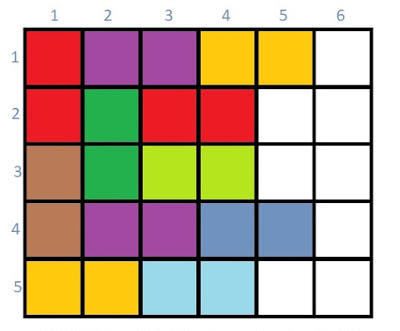
\includegraphics[width=0.5\linewidth]{img/counting_tiling_1}
	\caption{Relleno válido de las primeras 4 columnas dejando la quinta columna con el perfil 9, es decir, 01001}
	\label{fig:countingtiling1}
\end{figure}

\begin{figure}[!h]
	\centering
	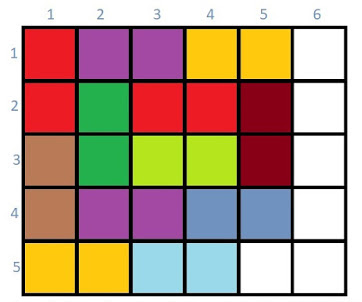
\includegraphics[width=0.5\linewidth]{img/counting_tiling_2}
	\caption{Relleno no válido que no se puede contar en dp[4][5] ya que el dominó marrón no se utiliza para rellenar ninguna de las primeras cuatro columnas. Nota: 15 representa 01111, es decir, el perfil de la quinta columna}
	\label{fig:countingtiling2}
\end{figure}

Pero ¿cómo obtenemos la relación entre los estados? Una forma es obtener el valor de \(dp[i][p]\) de \(dp[i-1][q]\) expresando el primero como la suma de todos \(dp[i-1] [q]\) para lo cual existe un relleno de la \((i)\)ésima columna con fichas de dominó, dejando la \(i+1\)ésima columna con el perfil \(p\). La complejidad del tiempo para calcular \(dp[i][p]\) es igual a \(O(2^n)\). Como hay \(m \times 2^n\) estados, la complejidad del tiempo total se vuelve igual a \(O(m \times 2^{2n})\).


Pero obtendríamos un veredicto de TLE para el algoritmo anterior. Para evitar esto, en lugar de encontrar todos los perfiles posibles \(q\) tales que \(dp[i-1][q]\) pueda producir \(dp[i][p]\), para un perfil determinado \( q\) encontramos todos los perfiles posibles \(p\) tales que \(dp[i-1][q]\) pueda producir \(dp[i][p]\) y sumamos el valor de \(dp[ i-1][q]\) a \(dp[i][p]\). Esto significa que verificamos todas las formas posibles de llenar la \(i\)ésima columna que tiene el perfil \(q\). Para hacer esto, analicemos la \(i\)ésima columna desde el \(1\)er bloque de la columna hasta el \(n\)ésimo bloque de la columna.

Si el \(j\)ésimo bloque ya está ocupado por alguna ficha de dominó, entonces no hagas nada.
De lo contrario, este bloque se puede completar como máximo de dos maneras, como se detalla a continuación.

\begin{enumerate}
	\item Coloque una ficha de dominó en los bloques \((i,j)\) y \((i+1,j)\) y márquelos como ocupados.
	\item Coloque una ficha de dominó en los bloques \((i,j)\) y \((i,j+1)\) y márquelos como ocupados si el bloque (\(j+1)\) existe y está desocupado.
\end{enumerate}

Cada permutación que llena la columna actual produce un perfil único \(p\) que representa la \((i+1)\)ésima columna. Entonces agregamos \(dp[i][q]\) a \(dp[i+1][p]\) donde \(q\) es el perfil de la \(i\)ésima columna antes del llenado.

Ahora, observe que para \(i = 0\), llenar las primeras \(0\) columnas completamente y tener el perfil \(p\) para la \(1\)st columna es posible si \(p = 0\). Esto implica que \(dp[0][p]\) es igual a \(1\) para \(p = 0\) e igual a \(0\) para todo \(p \neq 0\).

Dado que necesitamos llenar todas las \(m\) columnas con el perfil para la \((m+1)\)ésima columna igual a 0 (ya que no existe ninguna \((m+1)\)ésima columna), el requerido la respuesta es igual a \(dp[m][0]\).

\subsection{Fórmula}
Como nota final, también existe una sorprendente fórmula directa para calcular el número de mosaicos, pero como la respuesta es un producto de números reales, un problema al usar la fórmula es cómo almacenar los resultados intermedios con precisión.La fórmula es la siguiente

$$ \prod_{a=1}^{\lceil n/2 \rceil } \prod_{b=1}^{\lceil m/2 \rceil } 4  (\cos^2 \frac{\pi a}{n+1} + \cos^2 \frac{\pi b}{m+1}) $$
\section{Implementación}
\subsection{C++}
\begin{lstlisting}[language=C++]
int n,m;
vector< vector<long long> > dp;

void tiling(int x=0, int y=0, int mask=0, int next_mask=0){
   if(x==n) return;
   if(y>=m) dp[x+1][next_mask]=dp[x+1][next_mask]+dp[x][mask];
   else{
      int my_mask=1<<y;
      if(mask & my_mask) tiling(x,y+1,mask,next_mask);
      else{
         tiling(x,y+1,mask,next_mask|my_mask);
         if(y+1<m && !(mask&my_mask) && !(mask&(my_mask<<1)))
         	tiling(x,y+2,mask,next_mask);
      }
   }
}

long long countTilings(int n,int m){
   dp.resize (n+1, vector<long long> (1<<m));
   dp[0][0]= 1;
   for (int x=0; x<=n; ++x)
      for (int mask=0; mask<(1<<m); ++mask)
         tiling(x, 0, mask, 0);
   return dp[n][0];
}
\end{lstlisting}
\subsection{Java}
\begin{lstlisting}[language=Java]
public static void tiling(int x, int y, int mask, int next_mask, long [] [] dp,int n,int m){
   if(x==n) return;
   if(y>=m) dp[x+1][next_mask]=dp[x+1][next_mask]+dp[x][mask];
   else{
      int my_mask=1<<y;
      if((mask & my_mask)>0) tiling(x,y+1,mask,next_mask,dp,n,m);
      else{
         tiling(x,y+1,mask,next_mask|my_mask,dp,n,m);
         if(y+1<m && !((mask & my_mask)>0) && !(( (mask & (my_mask<<1)) >0)))
            tiling(x,y+2,mask,next_mask,dp,n,m);
      }
   }
}

public static long countTilings(int n,int m){
   long [] [] dp =new long [n+1][1<<m];
   dp[0][0]= 1;
   for (int x=0; x<=n; ++x)
      for (int mask=0; mask<(1<<m); ++mask)
         tiling(x, 0, mask, 0,dp,n,m);
   return dp[n][0];
}
\end{lstlisting}
\section{Aplicaciones}
Contar mosaicos tiene varias aplicaciones en escenarios del mundo real, que incluyen:

\begin{enumerate}
\item \textbf{Diseño de interiores:} contar los mosaicos puede ayudar a determinar la cantidad de mosaicos necesarios para cubrir un área específica, como el piso o la pared, en una habitación. Esta información es crucial para estimar costos y planificar diseños de mosaicos.

\item \textbf{Arquitectura y construcción:} El conteo de los mosaicos es fundamental para calcular la cantidad de mosaicos necesarios para proyectos de gran envergadura, como fachadas de edificios o espacios públicos. Garantiza una estimación precisa del material y ayuda a optimizar el pedido y el almacenamiento de losetas.

\item \textbf{Resolución de acertijos:} las técnicas de conteo de mosaicos se utilizan a menudo en juegos y desafíos de resolución de acertijos, donde los jugadores deben organizar mosaicos para formar patrones o formas específicas. La capacidad de contar el número de acuerdos posibles ayuda a los jugadores a elaborar estrategias y encontrar soluciones.

\item \textbf{Matemáticas y combinatoria:} los problemas de conteo de mosaicos brindan desafíos matemáticos interesantes que se pueden resolver utilizando diversas técnicas, como la recursividad, la programación dinámica o la generación de funciones. Estos problemas contribuyen al estudio de la combinatoria y las matemáticas discretas.

\item \textbf{Animación y gráficos por computadora:} las técnicas de mosaico de conteo se utilizan en animación y gráficos por computadora para generar patrones de mosaicos realistas y visualmente atractivos. Al comprender la cantidad de arreglos posibles, los diseñadores pueden crear texturas y fondos visualmente agradables.
\end{enumerate}

En general, contar mosaicos juega un papel crucial en varios campos, desde aplicaciones prácticas en arquitectura y construcción hasta la resolución de problemas matemáticos y el diseño creativo.
\section{Complejidad}
Para una columna particular con \(k\) bloques vacíos, el peor tiempo de ejecución del análisis anterior es \(O(f_{k})\), donde \(f_{k}\) es \(k\) º número de Fibonacci. Hay \(^{n}C_{k}\) perfiles con \(k\) bloques vacíos. También hay columnas \(m\). Entonces, el tiempo total de ejecución es \(m \times \sum_{k = 0}^{n}\) \(^{n}C_{k} \times O(f_{k})\) que es igual a \(O(m \times (1+ \phi)^n)\). Observe que este algoritmo es muy eficiente que el anterior.
\section{Ejercicios}
A continuación una lista de ejercicios que se pueden resolver aplicando el algoritmo analizado en la presente guía:

\begin{itemize}
	\item \href{https://cses.fi/problemset/task/2181}{CSES - Counting Tilings}
	\item \href{https://dmoj.uclv.edu.cu/problem/campipvc}{DMOJ - Tiling}
\end{itemize}

\end{document}